% System overview (fig:overview in sn-article.tex), 7.16 in x 2.4 in, sans-serif 8 pt.
% Overleaf: set this file as the main document, recompile, download the PDF, upload it as figures/fig_overview.pdf,
% then set sn-article.tex as the main document again. Locally: pdflatex fig_overview.tex in paper/.
% Thumbnails: figures/thumbs/thumb_{rgb,depth,coords}.png from make_thumbnails.py (training PC). Where a file does
% not exist, a schematic icon is drawn instead (room view, its depth, the coordinate grid), so the file always compiles
% and the figure is usable without the recordings.
\documentclass[border=1pt]{standalone}
\usepackage[T1]{fontenc}
\usepackage[scaled=0.92]{helvet}
\renewcommand{\familydefault}{\sfdefault}
\usepackage{amsmath,amssymb}
\usepackage{sansmath}
\usepackage{graphicx}
\usepackage{tikz}
\usetikzlibrary{arrows.meta,calc}

\definecolor{learn}{HTML}{2A78D6}     % learned block (ours)
\definecolor{geo}{HTML}{7F7F7F}       % geometry / reference grey
\definecolor{scan}{HTML}{9ECAE1}      % room-scan poses
\definecolor{sweep}{HTML}{08306B}     % sweep poses

\newcommand{\thumb}[4]{% file, width, height, fallback (schematic icon box)
  \IfFileExists{#1}{\includegraphics[width=#2,height=#3]{#1}}{#4}}

% ---- schematic icons, 1.55 cm x 0.872 cm (16:9), used when the real thumbnails are missing
% one room view: back wall with a window, side walls, floor, an examination couch and a cabinet
\newcommand{\roomgeom}{%
  \coordinate (bl) at (0.30,0.30); \coordinate (br) at (1.22,0.30);
  \coordinate (tl) at (0.30,0.872); \coordinate (tr) at (1.22,0.872);}
\definecolor{h1F5A9C}{HTML}{1F5A9C}\definecolor{h2D6FB0}{HTML}{2D6FB0}\definecolor{h3A7DBD}{HTML}{3A7DBD}
\definecolor{h5B7FA6}{HTML}{5B7FA6}\definecolor{h6BA3D3}{HTML}{6BA3D3}\definecolor{h6E6C67}{HTML}{6E6C67}
\definecolor{h7A9CC0}{HTML}{7A9CC0}\definecolor{h8C8A84}{HTML}{8C8A84}\definecolor{h9CC3E4}{HTML}{9CC3E4}
\definecolor{hB9B3A8}{HTML}{B9B3A8}\definecolor{hCFE3F2}{HTML}{CFE3F2}\definecolor{hD9D1C2}{HTML}{D9D1C2}
\definecolor{hDCD5C7}{HTML}{DCD5C7}\definecolor{hE4E4E4}{HTML}{E4E4E4}\definecolor{hE9E3D7}{HTML}{E9E3D7}
\newsavebox{\iconrgb}\newsavebox{\icondepth}\newsavebox{\iconcoords}
\sbox{\iconrgb}{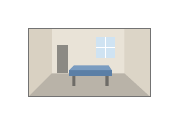
\begin{tikzpicture}[x=1cm,y=1cm]
  \roomgeom
  \fill[hE9E3D7] (0,0) rectangle (1.55,0.872);                               % back wall
  \fill[hD9D1C2] (0,0) -- (bl) -- (tl) -- (0,0.872) -- cycle;                % left wall
  \fill[hDCD5C7] (1.55,0) -- (br) -- (tr) -- (1.55,0.872) -- cycle;          % right wall
  \fill[hB9B3A8] (0,0) -- (1.55,0) -- (br) -- (bl) -- cycle;                 % floor
  \fill[hCFE3F2] (0.86,0.50) rectangle (1.10,0.76);                          % window
  \draw[white, line width=0.5pt] (0.98,0.50) -- (0.98,0.76) (0.86,0.63) -- (1.10,0.63);
  \fill[h8C8A84] (0.36,0.30) rectangle (0.50,0.66);                          % cabinet
  \fill[h6E6C67] (0.56,0.14) rectangle (0.60,0.27) (0.98,0.14) rectangle (1.02,0.27);  % couch legs
  \fill[h5B7FA6] (0.52,0.27) rectangle (1.06,0.34);                          % couch front
  \fill[h7A9CC0] (0.52,0.34) -- (1.06,0.34) -- (1.02,0.40) -- (0.58,0.40) -- cycle;    % couch top
  \draw[black!55, line width=0.4pt] (0,0) rectangle (1.55,0.872);
\end{tikzpicture}}
% its depth: near = dark, far = light, no depth (window glass) = light grey
\sbox{\icondepth}{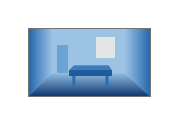
\begin{tikzpicture}[x=1cm,y=1cm]
  \roomgeom
  \fill[h9CC3E4] (0,0) rectangle (1.55,0.872);
  \shade[left color={rgb,255:red,33;green,102;blue,172}, right color={rgb,255:red,156;green,195;blue,228}]
    (0,0) -- (bl) -- (tl) -- (0,0.872) -- cycle;
  \shade[right color={rgb,255:red,33;green,102;blue,172}, left color={rgb,255:red,156;green,195;blue,228}]
    (1.55,0) -- (br) -- (tr) -- (1.55,0.872) -- cycle;
  \shade[bottom color={rgb,255:red,8;green,48;blue,107}, top color={rgb,255:red,140;green,184;blue,222}]
    (0,0) -- (1.55,0) -- (br) -- (bl) -- cycle;
  \fill[hE4E4E4] (0.86,0.50) rectangle (1.10,0.76);                          % no depth on glass
  \fill[h6BA3D3] (0.36,0.30) rectangle (0.50,0.66);
  \fill[h2D6FB0] (0.56,0.14) rectangle (0.60,0.27) (0.98,0.14) rectangle (1.02,0.27);
  \fill[h1F5A9C] (0.52,0.27) rectangle (1.06,0.34);
  \fill[h3A7DBD] (0.52,0.34) -- (1.06,0.34) -- (1.02,0.40) -- (0.58,0.40) -- cycle;
  \draw[black!55, line width=0.4pt] (0,0) rectangle (1.55,0.872);
\end{tikzpicture}}
% one room coordinate per cell, x, y, z shown as R, G, B
\sbox{\iconcoords}{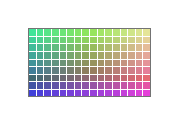
\begin{tikzpicture}[x=1cm,y=1cm]
  \foreach \i in {0,...,15}{\foreach \j in {0,...,8}{
    \pgfmathsetmacro{\r}{0.25+0.65*\i/15}
    \pgfmathsetmacro{\g}{0.25+0.65*\j/8}
    \pgfmathsetmacro{\b}{\j<3 ? 0.85-0.2*\j : 0.35+0.25*abs(\i-7.5)/7.5}
    \definecolor{cc}{rgb}{\r,\g,\b}
    \fill[cc] (\i*0.096875,\j*0.096889) rectangle ++(0.096875,0.096889);}}
  \draw[white, line width=0.15pt, step=0.096875] (0,0) grid (1.55,0.872);
  \draw[black!55, line width=0.4pt] (0,0) rectangle (1.55,0.872);
\end{tikzpicture}}

\begin{document}
\sansmath
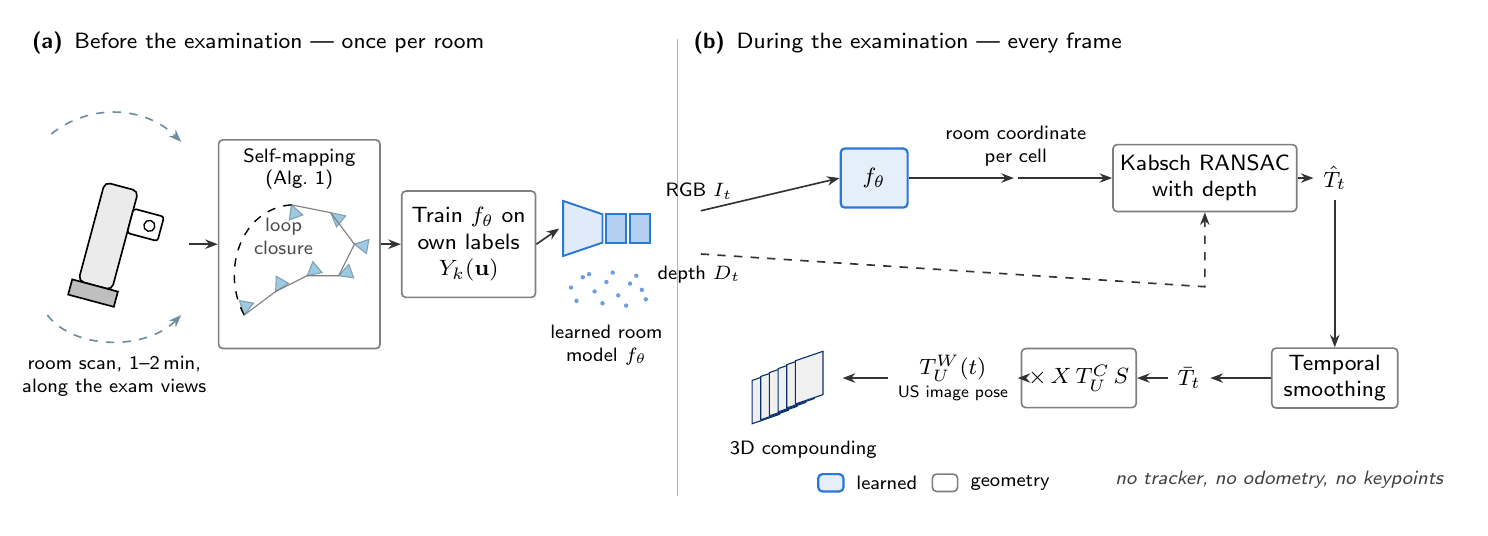
\begin{tikzpicture}[
    x=1cm, y=1cm,
    font=\fontsize{8}{9.5}\selectfont,
    small/.style={font=\fontsize{7}{8.2}\selectfont},
    arr/.style={-{Stealth[length=1.6mm,width=1.2mm]}, line width=0.6pt, draw=black!80},
    darr/.style={arr, dashed},
    geobox/.style={draw=geo, line width=0.6pt, rounded corners=1.5pt, fill=white, align=center, inner sep=2.5pt},
    learnbox/.style={draw=learn, line width=0.8pt, rounded corners=1.5pt, fill=learn!12, align=center, inner sep=2.5pt},
  ]
  % canvas 18.19 cm x 6.1 cm
  \path[use as bounding box] (0,0) rectangle (18.19,6.1);
  \draw[geo!60, line width=0.4pt] (8.25,0.15) -- (8.25,5.95);

  % ============================================================ (a) before the examination
  \node[anchor=north west, inner sep=0] at (0.05,6.05) {\textbf{(a)}\enspace Before the examination --- once per room};

  % (1) probe with the RGB-D camera, moved in the air along the sweep paths
  \begin{scope}[shift={(1.05,3.55)}, rotate=-15]
    \draw[line width=0.6pt, fill=black!8, rounded corners=2pt] (-0.22,-0.75) rectangle (0.22,0.55);   % handle
    \draw[line width=0.6pt, fill=black!25] (-0.30,-0.95) rectangle (0.30,-0.75);                       % transducer face
    \draw[line width=0.6pt, fill=white, rounded corners=1pt] (0.22,0.0) rectangle (0.62,0.32);         % camera
    \draw[line width=0.5pt] (0.47,0.16) circle (0.07);
  \end{scope}
  \draw[darr, scan!70!black] (0.25,2.45) .. controls (0.6,2.0) and (1.5,2.0) .. (1.95,2.45);
  \draw[darr, scan!70!black] (0.30,4.75) .. controls (0.8,5.15) and (1.5,5.1) .. (1.95,4.65);
  \node[small, align=center, anchor=north] at (1.1,2.05) {room scan, 1--2\,min,\\along the exam views};

  % (2) self-mapping: camera frusta along a path, one loop closure
  \node[geobox, minimum width=2.05cm, minimum height=2.65cm] (map) at (3.45,3.35) {};
  \node[small, anchor=north, align=center] at (map.north) {Self-mapping\\(Alg.~1)};
  \foreach \x/\y/\a in {2.75/2.45/80, 3.15/2.75/60, 3.55/2.95/40, 3.95/2.95/20, 4.15/3.35/-10, 3.85/3.75/-40, 3.35/3.85/-70}{
    \begin{scope}[shift={(\x,\y)}, rotate=\a]
      \draw[scan!80!black, fill=scan, line width=0.4pt] (0,0) -- (0.17,0.09) -- (0.17,-0.09) -- cycle;
    \end{scope}}
  \draw[geo, line width=0.4pt] (2.75,2.45) -- (3.15,2.75) -- (3.55,2.95) -- (3.95,2.95) -- (4.15,3.35) -- (3.85,3.75) -- (3.35,3.85);
  \draw[dashed, learn!0!black, line width=0.5pt] (3.35,3.85) .. controls (2.7,3.8) and (2.45,3.0) .. (2.75,2.45);
  \node[small, align=center, text=black!70] at (3.25,3.45) {loop\\closure};

  % (3) training on own labels
  \node[geobox, minimum width=1.7cm, minimum height=1.35cm] (train) at (5.6,3.35)
    {Train $f_\theta$ on\\own labels\\$Y_k(\mathbf{u})$};

  % (4) learned room model
  \begin{scope}[shift={(7.35,3.55)}]
    \draw[learn, line width=0.7pt, fill=learn!15] (-0.55,0.35) -- (-0.05,0.18) -- (-0.05,-0.18) -- (-0.55,-0.35) -- cycle;
    \draw[learn, line width=0.7pt, fill=learn!35] (0.0,0.18) rectangle (0.25,-0.18);
    \draw[learn, line width=0.7pt, fill=learn!35] (0.3,0.18) rectangle (0.55,-0.18);
    \foreach \px/\py in {-0.45/-0.75, -0.3/-0.62, -0.15/-0.8, 0.0/-0.68, 0.15/-0.85, 0.3/-0.7, 0.45/-0.78,
                        -0.38/-0.92, -0.05/-0.95, 0.25/-0.98, 0.5/-0.9, -0.22/-0.58, 0.08/-0.56, 0.38/-0.6}
      \fill[learn!70] (\px,\py) circle (0.028);
  \end{scope}
  \node[small, align=center, anchor=north] at (7.35,2.45) {learned room\\model $f_\theta$};

  \draw[arr] (2.05,3.35) -- (map.west);
  \draw[arr] (map.east) -- (train.west);
  \draw[arr] (train.east) -- (6.75,3.55);

  % ============================================================ (b) during the examination
  \node[anchor=north west, inner sep=0] at (8.45,6.05) {\textbf{(b)}\enspace During the examination --- every frame};

  % row 1: inputs -> network -> coordinates -> Kabsch
  \node[inner sep=0, anchor=south west] (rgb) at (8.5,3.75) {\thumb{figures/thumbs/thumb_rgb.png}{1.55cm}{0.872cm}{\usebox{\iconrgb}}};
  \node[small, anchor=south] at (rgb.north) {RGB $I_t$};
  \node[inner sep=0, anchor=north west] (dep) at (8.5,3.25) {\thumb{figures/thumbs/thumb_depth.png}{1.55cm}{0.872cm}{\usebox{\icondepth}}};
  \node[small, anchor=north] at (dep.south) {depth $D_t$};

  \node[learnbox, minimum width=0.85cm, minimum height=0.75cm] (net) at (10.75,4.19) {$f_\theta$};
  \node[inner sep=0] (coords) at (12.55,4.19) {\thumb{figures/thumbs/thumb_coords.png}{1.55cm}{0.872cm}{\usebox{\iconcoords}}};
  \node[small, anchor=south, align=center] at (coords.north) {room coordinate\\per cell};
  \node[geobox, minimum width=1.75cm, minimum height=0.85cm] (kabsch) at (14.95,4.19) {Kabsch RANSAC\\with depth};
  \node (That) at (16.6,4.19) {$\hat T_t$};

  \draw[arr] (rgb.east) -- (net.west);
  \draw[arr] (net.east) -- (coords.west);
  \draw[arr] (coords.east) -- (kabsch.west);
  \draw[arr] (kabsch.east) -- (That.west);
  \draw[darr] (dep.east) -- (14.95,2.81) -- (kabsch.south);

  % row 2 (right to left): smoothing -> US image pose -> compounding
  \node[geobox, minimum width=1.6cm, minimum height=0.75cm] (smooth) at (16.6,1.65) {Temporal\\smoothing};
  \node (Tbar) at (14.75,1.65) {$\bar T_t$};
  \node[geobox, minimum width=1.2cm, minimum height=0.75cm] (calib) at (13.35,1.65) {$\times\, X\,T^{C}_{U}\,S$};
  \node[align=center] (Tus) at (11.75,1.65) {$T^{W}_{U}(t)$\\[-1pt]{\fontsize{6.5}{7.5}\selectfont US image pose}};
  % small compounded volume
  \begin{scope}[shift={(9.65,1.42)}]
    \foreach \i in {0,...,5}{
      \draw[sweep, line width=0.4pt, fill=black!6] ($(-0.45,-0.35)+(\i*0.11,\i*0.05)$) -- ++(0,0.55) -- ++(0.35,0.12) -- ++(0,-0.55) -- cycle;}
  \end{scope}
  \node[small, anchor=north] at (9.85,0.98) {3D compounding};

  \draw[arr] (That.south) -- (smooth.north);
  \draw[arr] (smooth.west) -- (Tbar.east);
  \draw[arr] (Tbar.west) -- (calib.east);
  \draw[arr] (calib.west) -- (Tus.east);
  \draw[arr] (Tus.west) -- (10.35,1.65);

  \node[small, anchor=south east, font=\fontsize{7}{8.2}\selectfont\itshape, text=black!75] at (18.1,0.12)
    {no tracker, no odometry, no keypoints};

  % legend
  \begin{scope}[shift={(13.1,0.32)}]
    \node[learnbox, minimum width=0.32cm, minimum height=0.22cm, inner sep=0] at (-2.9,0) {};
    \node[small, anchor=west] at (-2.7,0) {learned};
    \node[geobox, minimum width=0.32cm, minimum height=0.22cm, inner sep=0] at (-1.45,0) {};
    \node[small, anchor=west] at (-1.25,0) {geometry};
  \end{scope}
\end{tikzpicture}
\end{document}
